\documentclass[11pt]{report}
\usepackage[english, russian]{babel}
\usepackage{xltxtra}
\usepackage{polyglossia}
\usepackage{mathpazo}

\defaultfontfeatures{Ligatures=TeX,Mapping=tex-text}

\setmainfont{STIX2Text-Regular.otf}[
ExternalLocation={stix2font/},
BoldFont=STIX2Text-Bold.otf,
ItalicFont=STIX2Text-Italic.otf,
BoldItalicFont=STIX2Text-BoldItalic.otf
]
\setmathrm{STIX2Math.otf}[
ExternalLocation={stix2font/}
]


\usepackage{makeidx}
\usepackage{amssymb, amsthm, amsfonts}
\usepackage{amsmath}
\usepackage{mathtools}
\usepackage{needspace}
\usepackage{enumitem}
\usepackage{fdsymbol}
\usepackage{fontawesome}


% разметка страницы и колонтитул
\usepackage[left=1.5cm,right=2cm,top=1.5cm,bottom=1.1cm,bindingoffset=0cm]{geometry}
\usepackage{fancybox,fancyhdr}
\fancyhf{}
\fancyhead[R]{\thepage}
\fancyhead[L]{\rightmark}
\fancyfoot{}
\fancyhfoffset{0pt}
\addtolength{\headheight}{13pt}
\pagestyle{fancy}

% Отступы
\setlength{\parindent}{3ex}
\setlength{\parskip}{3pt}

\usepackage{graphicx}
\usepackage{hyperref}

\usepackage{import}
\usepackage{xifthen}
\usepackage{pdfpages}

\newcommand{\incfig}[1]{%
    \def\svgwidth{\columnwidth}
    \import{./figures/}{#1.pdf_tex}
}


\usepackage{xifthen}
\makeatother
\def\@lecture{}%
\newcommand{\lecture}[3]{
    \ifthenelse{\isempty{#3}}{%
        \def\@lecture{Лекция #1}%
    }{%
        \def\@lecture{Лекция #1: #3}%
    }%
    \subsection*{\@lecture}
    \marginpar{\small\textsf{\mbox{#2}}}
}
\makeatletter


\usepackage{xcolor}
\definecolor{Aquamarine}{cmyk}{50, 0, 17, 100}
\definecolor{ForestGreen}{cmyk}{76, 0, 76, 45}
\definecolor{Pink}{cmyk}{0, 100, 0, 0}
\definecolor{Cyan}{cmyk}{56, 0, 0, 100}
\definecolor{Gray}{gray}{0.3}


 % Цвета для гиперссылок
\definecolor{linkcolor}{HTML}{3f888f} % цвет ссылок
\definecolor{urlcolor}{HTML}{af0000} % цвет гиперссылок
 
\hypersetup{pdfstartview=FitH,  linkcolor=linkcolor,urlcolor=urlcolor, colorlinks=true}


\usepackage{mdframed}
\mdfsetup{skipabove=3pt,skipbelow=3pt}
\mdfdefinestyle{defstyle}{%
    linecolor=red,
	linewidth=1pt,leftline=true,topline=false,bottomline=false, rightline=false,%
    frametitlerule=false,%
    frametitlebackgroundcolor=red!0,%
    innertopmargin=0pt,innerbottommargin=4pt,innerleftmargin=7pt
    frametitlebelowskip=10pt,
    frametitleaboveskip=7pt,
}
\mdfdefinestyle{thmstyle}{%
    linecolor=cyan!100,
	linewidth=2pt,topline=false,bottomline=false,%
    frametitlerule=false,%
    frametitlebackgroundcolor=cyan!20,%
    innertopmargin=4pt,innerbottommargin=4pt,
    frametitlebelowskip=1pt,
    frametitleaboveskip=3pt,
}
\theoremstyle{definition}
\mdtheorem[style=defstyle]{defn}{Определение}

\newmdtheoremenv[nobreak=true,backgroundcolor=Aquamarine!10,linewidth=0pt,innertopmargin=0pt,innerbottommargin=7pt]{cor}{Следствие}
\newmdtheoremenv[nobreak=true,backgroundcolor=CarnationPink!20,linewidth=0pt,innertopmargin=0pt,innerbottommargin=7pt]{desc}{Описание}
\newmdtheoremenv[nobreak=true,backgroundcolor=Gray!10,linewidth=0pt,innertopmargin=0pt,innerbottommargin=7pt,font={\small}]{ex}{Пример}
\newmdtheoremenv[nobreak=false,backgroundcolor=cyan!10,linewidth=0pt,innertopmargin=0pt,innerbottommargin=7pt]{thm}{Теорема}
\newmdtheoremenv[nobreak=true,backgroundcolor=Pink!10,linewidth=0pt,innertopmargin=0pt,innerbottommargin=7pt]{lm}{Лемма}

\newtheorem*{st}{Утверждение}
\newtheorem*{prop}{Свойства}

\theoremstyle{plain}
\newtheorem*{name}{Обозначение}

\theoremstyle{remark}
\newtheorem*{rem}{Ремарка}
\newtheorem*{com}{Комментарий}
\newtheorem*{note}{Замечание}
\newtheorem*{prac}{Упражнение}
\newtheorem*{probl}{Задача}


\renewcommand{\proofname}{Доказательство}
\renewenvironment{proof}
{ \hspace{\stretch{1}}\\ \faSquareO\quad  }
{ \hspace{\stretch{1}}  \faSquare }

\newenvironment{proof*}
{ \hspace{\stretch{1}}\\ {\color{orange}\faSquareO}\quad  }
{ \hspace{\stretch{1}}  {\color{orange}\faSquare} }


\numberwithin{ex}{section}
\numberwithin{thm}{section}
\numberwithin{equation}{section}



\newcommand{\A}{\mathcal{A}}
\newcommand{\K}{\mathcal{K}}
\newcommand{\Z}{\mathbb{Z}}
\newcommand{\N}{\mathbb{N}}
\newcommand{\Real}{\mathbb{R}}
\newcommand{\Q}{\mathbb{Q}}
\newcommand{\Cm}{\mathbb{C}}
\newcommand{\Pm}{\mathbb{P}}
\newcommand{\E}{\mathbb{E}}

\renewcommand{\o}{o}
\renewcommand{\O}{\mathcal{O}}

\renewcommand{\le}{\leqslant}
\renewcommand{\ge}{\geqslant}


\newcommand{\ord}{\operatorname{ord}}
\newcommand{\lcm}{\operatorname{lcm}}
\newcommand{\sign}{\operatorname{sign}}
\newcommand{\sg}{\operatorname{sg}}
\newcommand{\bsg}{\operatorname{\overline{sg}}}

\newcommand{\Div}{\operatorname{Div}}
\newcommand{\Prime}{\operatorname{Prime}}
\newcommand{\expp}{\operatorname{ex}}
\newcommand{\ith}{\operatorname{ith}}


\def\mybf#1{\textbf{#1}}
\def\selectedFont#1{\textbf{#1}}
\def\prf{\textbf{ПРФ}}
\def\crf{\textbf{ЧРФ}}
\def\orf{\textbf{ОРФ}}
\def\prec{п.р.}
\def\orec{о.р.}

\newcommand{\const}{\textmd{const}}
\newcommand{\R}{\mathbf{R}}
\renewcommand{\S}{\mathbf{S}}
\newcommand{\M}{\mathbf{M}}
\newcommand{\F}{\mathcal{F}}



\title{Конспект по теории вычислимости\\IV семестр, 2021 год\\
    Современное программирование, факультет математики и компьютерных наук, СПбГУ\\
(лекции Пузыниной Светланы Александровны)}
\author{Тамарин Вячеслав}

\makeindex
\begin{document}
\maketitle
\tableofcontents
\hspace{1em}
\begin{center}
	Исходный код на \url{https://github.com/tamarinvs19/theory_university}
\end{center}
\hspace{2em}
\begin{center}
	\textbf{
    Некоторые доказательства были опущены на лекции, но написаны мной. Они выделены оранжевыми символами:
}
	\begin{proof*}
		Исправляйте, дополняйте, меняйте. Чем меньше недоказанных утверждений, тем лучше!
	\end{proof*}
\end{center}

\printindex
\chapter{Введение в теорию сложности вычислений}
\lecture{1}{5 nov}{\dag}

\section{Машины Тьюринга}
\subsection{Напоминания}
Обсудим, что мы решаем.
\begin{name}
	~\begin{itemize}[noitemsep]
		\item Алфавит будет бинарный  $\{0, 1\}$;
		\item Множество всех слов длины $ n$ : $ \{0, 1\}^{n}$;
		\item Множество всех слов конечной длины  $ \{0, 1\}^{*}$;
		\item Длина слова $ x\colon  \lvert x \rvert $.
	\end{itemize}
\end{name}

\begin{defn}
    \noindent
    \selectedFont{Язык}\index{язык} (задача распознавания, decision problem) ---  $ L \subseteq \{0, 1\}^{*}$.
	
    \noindent
    \selectedFont{Индивидуальная задача}\index{индивидуальная задача} --- пара,
	первым элементом которой является условие, а второй~-- решение;
	принадлежит $ \{0, 1\}^{*} \times \{0, 1\}^{*}$.
	
	\noindent
	\selectedFont{Массовая задача}\index{массовая задача} --- некоторое множество индивидуальных задач, то есть бинарное отношение на $ \{0, 1\}^{*}$.
\end{defn}

\begin{defn}
	Будем говорить, что алгоритм \selectedFont{решает задачу поиска} для массовой задачи $ R$, если для условия $ x$ он находит решение $ w$, удовлетворяющее $ (x, w) \in R$.

	\noindent
	Можем сопоставить массовой задаче, заданной отношением $ R$, язык
	\[
		L(R) = \{x \mid \exists w\colon (x, w) \in R\}
	.\]
\end{defn}

\begin{ex}[Массовая задача и соответствующий язык]
	\[
		\FACTOR = \{(n, d) \mid d | n, ~ 1<d<n\}
	.\]
	Здесь условием задачи является натуральное число  $ n$, а решением некоторый (не 1, и не $ n$) делитель числа $ n$.

	Данной задаче соответствует язык
	\[
		L(\FACTOR) = \text{множество всех составных чисел}
	.\]
\end{ex}

\subsection{Детерминированная машина Тьюринга}
\begin{defn}[Детерминированная машина Тьюринга]
	\selectedFont{Детерминированная машина Тьюринга}\index{машина Тьюринга детерминированная} ---
	\begin{itemize}[noitemsep]
		\item конечный алфавит (с началом ленты и пробелом): $ \Sigma  = \{0, 1, \triangleright, \_\}$;
		\item несколько лент, бесконечных в одну сторону;
		\item читающие/пишущие головки, по одной на каждую ленту;
		\item конечное множество состояний, в том числе начальное ($ q_S$/$q_0$), принимающее ($ q_Y $/$ q_{acc}$) и отвергающее ($ q_N$/$ q_{rej}$);
		\item управляющее устройство (программа), содержащее для каждых $ q, c_1, \ldots c_k$ одну инструкцию вида
			\[
				(q, c_1, \ldots c_k) \mapsto (q', c_1', \ldots c_k', d_1, \ldots d_k)
			,\]
			где $ q, q' \in Q$ --- состояния, $ c_i, c_i' \in \Sigma $ --- символы, обозреваемые головками, $ d_i \in \{ \to , \leftarrow, \cdot  \}$ --- направления движения головок.
	\end{itemize}

	ДМТ \selectedFont{принимает} входное слово, если заканчивает работу в $ q_{acc}$, и \selectedFont{отвергает}, если заканчивает в $ q_{rej}$.

	ДМТ $ M$ \selectedFont{распознает язык $ A$}, если принимает все $ x \in A$ и отвергает все $ x \not\in A$.
	\[
		A = L(M)
	.\]
\end{defn}
\begin{note}
	Обычно есть отдельная лента только для чтения, куда записаны входные данные, \\
	и лента только для вывода, куда нужно поместить ответ. Остальные ленты будут рабочими.
\end{note}
\begin{note}
	Изначально на входной ленте вход и пробелы, на остальных пробелы, головки в крайней левой позиции, а состояние есть $ q_s$.
\end{note}

\begin{defn}
	\selectedFont{Время работы  машины } \index{время работы МТ} $ M$ на входе $ x$ --- количество шагов (применений инструкций) \\ 
	до  достижения $ q_{acc}$ или $ q_{rej}$.

	\noindent
	\selectedFont{Используемая память} \index{используемая память} --- суммарное крайнее правое положение всех головок на \textit{рабочих} лентах.
\end{defn}

\begin{thm}\label{th:two_bands}
	Для любого $ k \in \N$, работу ДМТ  $ M$ с $ k$ рабочими лентами, работающую $ t$ шагов, можно  промоделировать на  ДМТ с двумя рабочими лентами за время  $ \O(t \log t)$,
	где константа $ \O(\ldots) $ зависит только от размеров записи машины $ M$.
\end{thm}
\begin{proof}
	\begin{itemize}
		\item
			Перестроим исходную МТ:
			\begin{itemize}
				\item Запишем все ленты в одну строку  по символу из всех лент по очереди.
				\item  Будем бегать <<лентой по головке>>: выровняем все ленты, чтобы головки стояли друг над  другом и далее будем сдвигать нужную ленту.
				\item Заметим, что двустороннюю ленту можно смоделировать на односторонней, причем
				с увеличением количества операций в константу раз: \\
				разрезаем двустороннюю пополам и записываем элементы через один.
			\end{itemize}
			\begin{figure}[ht]
				\centering
				\incfig{two-bands}
				\caption{Построение новой МТ}
				\label{fig:two-bands}
			\end{figure}
		\item
			Теперь поймем, как экономично сдвигать ленты в однострочной записи.

			Разобьем строку на блоки начиная от позиции головки в две стороны: справа блоки $ R_i$, слева $ L_i$. При этом $ \lvert L_i \rvert = \lvert R_i \rvert  = 2^{i}$. Раздвинем символы, заполняя пустоту специальными символами пустоты, так, чтобы в каждом блоке ровно половина элементов были пустыми.

			Далее будем поддерживать такое условие:
			\begin{enumerate}[noitemsep]
				\item В блоке либо информация, либо пусто, либо наполовину (ровно) пусто
				\item $ L_i$ пустой, когда  $ R_i$ полный
				\item  $ L_i$ наполовину пустой, когда $ R_i$ наполовину полный
				\item $ L_i$ полный, когда $ R_i$ пустой
			\end{enumerate}

			Пусть нужно подвинуть головку влево. Найдем слева первый не пустой блок $ L_i$. Возьмем из него правую половину и разложим по пустым $ L_{<i}$ так, чтобы порядок сохранился и каждый из $ L_{<i}$ стал полупустым, а первый символ попал под головку.

			Так получится сделать, так как всего перемещаемых символов $ 2^{i-1}$, а в $ j$-й блок будет помещено $ 2^{j-1}$ символов, поэтому всего в $ L_{<i}$ поместится
			\[
				1 + 2 + 4 + \ldots + 2^{i-2} = 2^{i-1} - 1
			.\]
			И один символ под головку.

			Чтобы инвариант сохранился нужно теперь исправить правую часть.

			Так как первые $ i-1$ левых блоков были пусты, первые $ i-1$ правых блоков полны, а $ R_i$ пуст (либо наполовину полон, в зависимости от первоначального состояния $ L_i$).
			Заполним половину в $ R_i$ символами из $ R_{i-1}$.
			Теперь $ R_{i-1}$ пустой, а меньшие полные. Проделаем ту же операцию еще раз для $ i-1$, потом для $ i-2$ и так далее. Заметим, что по отношению к $ R_i$ все сохранилось: если $ L_i$ был наполовину полон, то стал пуст, а $ R_i$ - полон (так как до этого  был наполовину полон). Полностью аналогичный случай, если бы $ L_i$ был полон.

			Когда мы дойдем до $ R_1$, положим туда элемент из-под головки.

			Итого, инвариант  сохранился.
			\begin{figure}[ht]
				\centering
				\incfig{blocks}
				\caption{Структура блоков}
				\label{fig:blocks}
			\end{figure}
		\item Посчитаем количество операций. В алгоритме переносим различные отрезки из одного места в другое. Чтобы делать это за линию, сначала скопируем нужный участок на вторую ленту, а затем запишем с нее.

			Тогда при перераспределении происходит $ c\cdot 2^{i}$ операций: \\ 
			каждый символ переносили константное число раз (на вторую ленту, со второй ленты)  плюс линейное перемещение от $ L_i$ к $ R_i$ несколько раз (символов всего $ 2^{i - 1}$ в каждой половине, итого суммарно перенесли $ 2^i$ символов).

			Докажем, что с $ i$-м блоком происходят изменения не чаще $ 2^{i-1}$  шагов. Пусть $ L_i$ хотя бы наполовину заполнен. Когда мы забрали половину из него, мы заполнили все $ L_{<i}$ и $ R_{<i}$ наполовину.

			Поэтому, чтобы изменить $ L_i$ еще раз, нужно сначала опустошить все $ L_{<i}$.
			При перераспределении в левой части становится на один элемент меньше, а всего там $ 2^{i-1}$ заполненное место. Для того, чтобы все они ушли из левой половины, придется совершить $ 2^{i-1}$ сдвигов.

			Итого, для $ t$ шагов исходной машины будет
			\[
				\sum_{i}^{\log t}c\cdot 2^{i} \cdot \frac{t}{2^{i-1}} = \O(t \log t)
			.\]
			Почему сумма до логарифма? Заметим, что так как мы сделали не более чем $ t$ шагов изначально, то мы не можем на каждой ленте занять более чем $ t$ ячеек. В таком случае, самый большой блок не будет больше $ t$. А его индекс, соответственно не будет больше, чем $ \log t$.
			\begin{note}
			Так как до этого у нас было k лент и все сдвиги делались одновременно, то здесь мы делаем сдвиг каждой ленты по очереди. То есть на самом деле мы получаем $ \O(k \cdot t \log t)$, но $ k$ в данном случае просто константа (почти точно константа может стать намного больше, чем $ k$, но всё равно останется константой). 
			\end{note}
	\end{itemize}
\end{proof}

\begin{thm}[Об универсальной МТ]
	Существует ДМТ $ U$, выдающая на входе $(M, ~ x)$ тот же результат, что дала бы машина $ M$ на входе $ x$, за время $ \O(t \log t)$, где $ t $ --- время работы $ M$ на входе $ x$.
\end{thm}
\begin{proof}
	Используем прием из прошлой теоремы \ref{th:two_bands}.
\end{proof}

\begin{note}
	Единственный способ узнать результат машины $M$ на строке $x$, это промоделировать вычисление машины $M$ на входе. Мы никогда не можем заранее сказать результат этого вычисления, и заканчивается ли оно вообще. Поэтому, моделировать вычисления (т.е. иметь универсальную машину Тьюринга) можно, но, например, нельзя иметь машину, которая по записи машины $M'$ скажет, принимает ли $M'$ пустую строку, можно лишь повести себя как $M'$ на пустой строке.
\end{note}

\section{Классы сложности}
\subsection{Классы $\DTIME$ и $\P$}

\begin{defn}[Конструируемая по времени функция]\index{конструируемая по времени функция}
	Функция $ t\colon \N \to  \N$ называется \selectedFont{конструируемой по времени}, если
	\begin{itemize}[noitemsep]
		\item $ t(n) \ge n$;
		\item двоичную запись  $ t(\lvert x \rvert )$ можно найти по входу $ x$ на ДМТ за  $ t(\lvert x \rvert )$ шагов.
	\end{itemize}
\end{defn}

\begin{note}
    Все стандартные функции (многочлены, экспоненты) конструируемы по времени. 
    
    Неконструируемыми являются вырожденные, специально построенные случаи.
\end{note}

\begin{defn}[Класс $\DTIME$]\index{$\DTIME$}
	Язык $ L$ принадлежит классу $ \DTIME[t(n)]$, если существует ДМТ $ M$, принимающая $ L$ за время $ \O(t(n))$, где $ t$ конструируема по времени.

	\noindent
	Константа может зависеть от языка, но не от длины входа.
\end{defn}

\begin{defn}[Класс $\P$]\index{$\P$}
	Класс языков, распознаваемых за полиномиальное время на ДМТ ---
	\[
		\P = \bigcup_{c}^{} \DTIME[n^{c}]
	.\]
\end{defn}
Будем обозначать задачи, заданные отношениями волной.

\begin{defn}
	Массовая задача $ R$ \selectedFont{полиномиально ограничена}\index{полиномиально ограниченная задача}, если существует полином $ p$, ограничивающий длину кратчайшего решения:
	\[
		\forall x ~ \Bigl( \exists u \colon (x, u) \in  R \Longrightarrow \exists w \colon \bigl( (x, w) \in R \wedge \lvert w \rvert \le p(\lvert x \rvert )\bigr)\Bigr)
	.\]
	Массовая задача $ R$ \selectedFont{полиномиально проверяема}\index{полиномиально проверяемая задача}, если существует полином $ q$, ограничивающий время проверки решения: для любой пары $ (x, w)$ можно проверить принадлежность $ (x, w) \stackrel{?}{\in} R$ за время $ q(\lvert (x, w) \rvert )$.
\end{defn}
\begin{defn}[Класс $ \tNP$]\index{$ \tNP$}
	$ {\tNP}$ --- класс задач поиска, задаваемых полиномиально ограниченными полиномиально проверяемыми массовыми задачами.
\end{defn}
\begin{defn}[Класс $ \tP $]\index{$\tP$}
	$ { \tP} $ --- класс задач поиска из $ { \tNP} $, разрешимых за полиномиальное время.

	\noindent
	То есть класс задач поиска, задаваемых отношениями $ R$, что для всех $ x \in \{0, 1\}^{*}$ за полиномиальное время можно найти $ w$, для которого $ (x, w) \in  R$.
\end{defn}
\[
	\boxed{\text{Ключевой вопрос теории сложности } { \tP}  \stackrel{?}{=} { \tNP}}
\]
\begin{defn}[Класс $\NP$]\index{$\NP$}
	$ \NP$~---  класс языков (задач распознавания),  задаваемых полиномиально ограниченными полиномиально проверяемыми массовыми задачами:
	\[
		\NP = \{L(R) \mid R \in { \tNP} \}
	.\]
\end{defn}
\begin{note}
	$ L \in \NP$, если существует массовая п.о.п.п.\footnote{полиномиально ограниченная полиномиально проверяемая} задача, такая, что
	\[
		\forall x \in \{0, 1\}^{*} \colon  x \in L \Longleftrightarrow \exists w \colon (x, w) \in R
	.\]
\end{note}

\begin{defn}[Класс $\P$]\index{\P}
	\P --- класс языков (задач распознавания), распознаваемых за полиномиальное время.
	\[
		\P = \{L(R) \mid R \in \tP\}
	.\]
\end{defn}
\begin{note}
	Очевидно, $ \P \subseteq \NP$.
\end{note}
\[
	\boxed{\text{Ключевой вопрос теории сложности } { \P}  \stackrel{?}{=} { \NP}}
\]
 
\lecture{2}{12 nov}{\dag}
\section{Недетерминированная машина Тьюринга}
\begin{defn}[Недетерминированная машина Тьюринга] \index{машина Тьюринга недетерминированная}
	\selectedFont{Недетерминированная машина Тьюринга} --- машина Тьюринга, допускающая более одной инструкции для данного состояния $ q \in Q$ и $ c_1, \ldots c_k \in \Sigma $, то есть для состояния  $ q $ и символа $ c$ функция  $ \delta $ будет многозначной.
\end{defn}

Из такого определения получаем \selectedFont{дерево вычислений} вместо последовательности состояний ДМТ.

Мы говорим, что НМТ \footnote{недетерминированная машина Тьюринга} \selectedFont{принимает} вход, если существует путь в дереве вычислений, \\ заканчивающийся принимающим состоянием.

\begin{st}
	В машины (ДМТ / НМТ) с заведомо ограниченным временем работы можно встроить {\sc будильник} и считать время вычислений на входах одной длины всегда \textsc{одинаковым}.
	Для этого можем просто записать на дополнительную ленту $ t(n)$ единиц и стирать по одной за ход. 
\end{st}

\begin{defn}[Эквивалентное определние НМТ]
	\selectedFont{Недетерминированная машина Тьюринга} --- ДМТ, у которой есть дополнительный аргумент (конечная подсказка $ w$ на второй ленте).
\end{defn}
\begin{proof}
	Докажем эквивалентность. Представим дерево вычисления как бинарное дерево и пронумеруем ребра из каждой вершины $ 0$ и $ 1$. Теперь запишем нужную принимающую ветку на ленту-подсказку.
	По подсказке можем построить дерево, где будет нужный путь.
\end{proof}
\begin{defn}\index{\NP}
    Еще одно определение класса $ \NP$ --- класс языков, принимаемых полиномиальными по времени НМТ.
\end{defn}

\section{Сведения и сводимости}
\begin{defn}[Сведение по Карпу]\index{сведение по Карпу}
	Язык $ L_1$  \selectedFont{сводится по Карпу} к языку $ L_2$, если существует полиномиально вычислимая функция $ f$ такая, что
	\[
		\forall x\colon x \in L_1 \Longleftrightarrow f(x) \in L_2
	.\] 
\end{defn}

\begin{defn}[Сведение по Левину]\index{сведение по Левину}
	Задача поиска (отношение) $ R_1$ \selectedFont{сводится по Левину} к задаче $ R_2$, если существуют функции $ f, g, h$ такие, что для всех  $ x_1, y_1, y_2$ верно
	\begin{itemize}
		\item $ R_1(x_1, y_1) \Longrightarrow R_2(f(x_1), g(x_1, y_1))$;
		\item $ R_1(x_1, h(f(x_1), y_2)) \Longleftarrow R_2(f(x_1), y_2)$;
		\item $ f, g, h$ полиномиально вычислимые.
	\end{itemize}
	\begin{note}
	    Первое условие нужно для того, чтобы образы каждого входа, имеющего решение первой задачи, имели решение и второй задачи.
	\end{note}
\end{defn}

\begin{thm}
	Классы $\P, \NP, \tP, \tNP$ замкнуты относительно этих сведений.
\end{thm}
\begin{proof}
	Рассмотрим $ R_2 \in \tP$ и $ R_1 \to R_2$. Тогда должно выполняться $ R_1 \in \tP$. Аналогично для $ \tNP$. 
    В обоих случаях $ R_2$ задано п.о.п.п. Если говорим про $ \tP$, то еще есть алгоритм, работающий за полиномиальное время.

	Что можно узнать про $ R_1$? Если есть решение для $ R_1$, то функция $ g$ дает решение $ R_2$, которое не на много длиннее.
	Еще есть $ h$, которая позволяет построить из решения $ R_2$ обратно построить решение $ R_1$.
	\begin{itemize}
		\item Пусть есть некоторое решение $ y_1$ для задачи $ R_1$. Для него можно получить некоторое решение $ R_2$ -- $ g(x_1, y_1)$.

	Так как $ R_2$ полиномиально ограничено, для него есть полиномиальное решение поменьше. Поэтому, когда оно будет возвращено функцией $ h$, исходное решение $ y_2$ тоже окажется коротким.

		\item Полиномиальная проверяемость проверяется аналогично.

		\item Про алгоритм: если есть алгоритм для $ R_2$ и $ x_1$, сначала перегоняем $ x_1 \to  f(x_1)$, далее применяем алгоритм, получаем $ y_2$, а далее, используя $ h$, перегоняем обратно в $ R_1$.
	\end{itemize}
\end{proof}

\begin{defn}[Оракульная МТ]\index{машина Тьюринга оракульная}
	\selectedFont{Оракульная МТ} --- МТ с доступом к оракулу, который за один шаг дает ответ на некоторый вопрос.
\end{defn}
\begin{name}
	При переходе в состояние $ q_{\text{in}}$ происходит <<фантастический переход>> в состояние $ q_{\text{out}}$, заменяющий содержимое некоторой ленты на ответ оракула.

	\noindent$ M^{B}$ --- оракульная машина $ M$, которой дали оракул $ B$. 
\end{name}

\begin{defn}[Сведение по Тьюрингу]\index{сведение по Тьюрингу}
	Язык или задача $ A$ \selectedFont{сводится по Тьюрингу} к $ B$, если существует оракульная машина полиномиальная по времени $ M^{\medblackcircle}$ такая, что $ M^{B}$ решает $ A$.

	\noindent
	Например, если  $ A$ ---  язык, $ A = L(M^{B})$.
\end{defn}
\begin{ex}
	Классы $\P$ и $\tP$ замкнуты относительно сведений по Тьюрингу. А $\NP$ и $\tNP$ могут быть незамкнуты: если $A = \UNSAT,~ B = \SAT$, $ M^{O}(x) = \overline{(x \in O)}$, и $ A$ сводится по Тьюрингу к $ B$, но $ B \in \NP$, a про $ A$ не известно.
\end{ex}

\subsection{Трудные и полные задачи}
\begin{defn}[Трудный и полные задачи]
	Задача $ A$ называется \selectedFont{трудной}\index{трудная задача} для класса $\Class$, если  $ \forall C \in \Class \colon C \to A$.

	\noindent
	Задача $ A$ называется \selectedFont{полной}\index{полная задача} для класса $ \Class$, если она трудная и принадлежит $ \Class$.
\end{defn}

\begin{thm}
    Если $ A$ --- \NP-трудная и $ A \in \P$, то $ \P = \NP$.
\end{thm}
\begin{cor}
    Если $ A$ --- \NP-полная, то $
    A \in \P \Longleftrightarrow \P = \NP
    $. 
\end{cor}

\subsubsection{Задача об ограниченной остановке}
\begin{defn}[\BH]\index{\BH, задача об ограниченной подстановке}
	Определим задачу об ограниченной остановке $ \tBH(\langle M, x, 1^{t} \rangle, w)$ \footnote{здесь $ 1^{t}$ --- служебные $ t$ единиц} так:
	дана НМТ $ M$ и вход $ x$, требуется найти такую подсказку $ w$, чтобы $ M$ распознавала $ x$ не более чем за $ t$ шагов.

	\noindent
	Соответствующая задача распознавания --- ответить, существует ли такая подсказка.
\end{defn}
\begin{thm}
    Задача об ограниченной остановке $ \tNP$-полная, а соответствующий язык \NP-полный.
\end{thm}
\begin{proof}
	\begin{itemize}
		\item Принадлежность $ \tNP$ и $ \NP$ следует из существования универсальной ДМТ, которая за $ \O(t \log t)$ промоделирует вычисление ДМТ, описание которой дано ей на вход.
		\item Проверим, что язык  $ \NP$-трудный.
			Пусть  язык $ L$ принадлежит $ \NP$, что равносильно существованию для соответствующего отношения $ R$ машины Тьюринга $ M^{*}(x, w)$, которая работает за $ \poly(\lvert x \rvert )$.

			Сведем $ L$ к задаче $ \BH$. Рассмотрим тройку $ \langle M^{*}, x, 1^{\poly(\lvert x \rvert )} \rangle$. 
			Пусть функция $ f(x)$ будет равна этой тройке.

			Если и только если существует подсказка $ w$ для тройки $ f(x) $ принадлежит $ \BH$, а наш язык $ L$ и определяется машиной $ M^{*}$. 
		\item Аналогично для задач поиска.
    \end{itemize}
\end{proof}

\subsection{Булевы схемы}
\begin{defn}[Булева схема]\index{булевы схемы}
	\selectedFont{Булева схема} --- ориентированный граф  без циклов,в вершинах которого записаны бинарные, унарные или нульарные операции над битами ($ \wedge, \vee, \oplus$), при этом есть специальные вершины-входы и вершины-выходы.
\end{defn}
\begin{defn}[\CircuitSat]\index{\CircuitSat}
	\[
		\tCircuitSat = \{(C, w) \mid C\text{ --- булева схема}, C(w) = 1\}
	.\] 
\end{defn}
Очевидно, что $ \CircuitSat \in \NP$.
Чтобы доказать $ \NP$-трудность, сведем $ \BH \to \CircuitSat$:
будем рисовать конфигурацию МТ на схемах.
\begin{itemize}
	\item Пусть каждый этаж системы --- конфигурация ДМТ. Всего этажей будет столько же, сколько шагов в МТ, то есть $ t$. Если в последнем этаже $ q_{acc}$, то результат $ 1$.
	\item Пересчет конфигураций: меняются только гейты рядом с положением головки. Выделим подсхему, которая должна по состоянию и элементу рядом с головкой получить новое состояние, положение головки и поменять элемент, то есть построить новый уровень с измененными элементами.

		Для хранения головки будем после каждого символа с ленты хранить $ d_i $ равное единице, если головка на символе $ c_i$ перед ним.

		Если $ d_i = 0$, то новый $ c_i' = c_i$, иначе нужно заменить   $ c_i$ на $ c_i'$ из программы МТ:
		\[
			(q, c_{i-1}, c_i, c_{i+1}, d_{i-1}, d_i, d_{i+1}) \mapsto (q', c_i', d_i') 
		.\] 
	\item Так как входная строка $ x$ нам дана, запаяем ее в схему. Тогда входом схемы останется подсказка $ w$ для НМТ, а выходом --- попадание в $ q_{acc}$.
\end{itemize}
Таким образом, мы по $ M, x, t$ построили схему $ C(w)$.
 
\lecture{3}{15 April}{\dag}
\subsection{Подсчет углов в графе}
\begin{figure}[h]
	\begin{minipage}{0.7\textwidth}
Рассмотрим ориентированный граф.

Назовем \textit{треугольником} тройку $ (x, y, z)$, если это цикл из трех вершин. \textit{Углом} назовем тройку  $ (x, y, z)$, если есть ребра  $ xy$ и $xz$, при этом  $ y $ может совпадать  $ z$.

\textbf{Чего в графе больше: углов или треугольников?}
	\end{minipage}
	\begin{minipage}{0.25\textwidth}
		\center{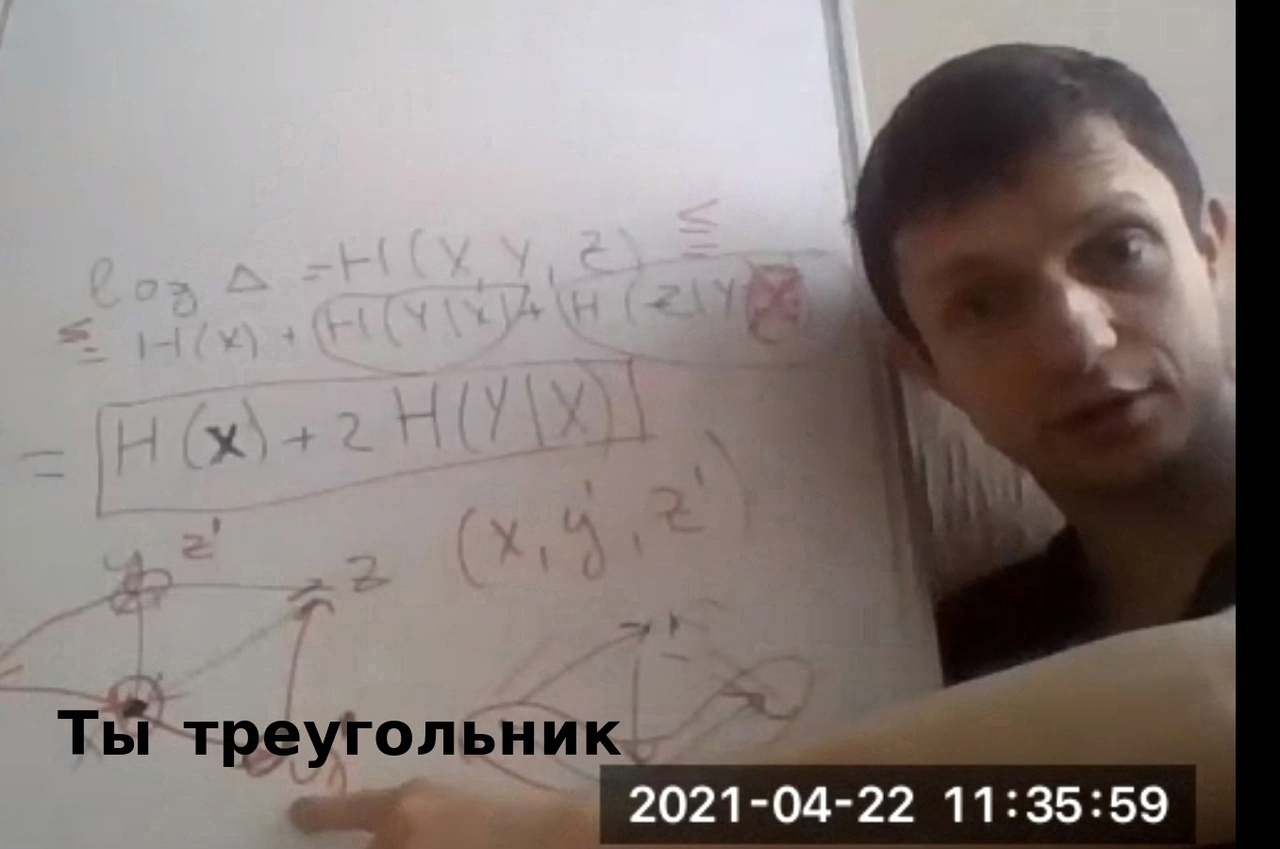
\includegraphics[width=\textwidth]{figures/you_are_triangle.jpg}}
	\end{minipage}
\end{figure}
\begin{note}
	Каждое ребро тоже угол, например, $ (x, y, y)$.
\end{note}
\begin{thm}
    Число углов в графе всегда больше числа треугольников.
\end{thm}
\begin{proof}
 	Пусть случная величина $ \alpha = (X, Y, Z)$ равна случайному треугольнику, где $ X, Y, Z$ --- с.в., соответствующие первой, второй и третьей вершине треугольника в равномерном распределении на треугольниках. 

	Так как распределение количества треугольников равномерно,
	\begin{align*}
		\log (\# \Delta)& = H(X, Y, Z)  = \\
					  &= H(X) + H(Y \mid  X) + H(Z \mid  Y, X) \le \tag{Chain rule}  \\
					  & \le  H(X) + H(Y \mid X) + H(Z \mid Y) = \tag{циклический сдвиг в треугольнике} \\
		 & = H(X) + 2 H(Y \mid X)
	\end{align*}
Найдем какое-то распределение на углах, энтропия которого хотя бы $ H(X) + 2H(Y \mid X)$, тогда эта сумма будет не более  $  \log (\# \angle)) $.
	% с картинкой будет лучше?

	Пусть мы выбрали случайный треугольник $ (x, y, z)$. Оставим $ x$ и выберем для него найдем случайный треугольник с $ x$ и возьмем из него следующую за $ x$ вершину $ y'$. Повторяем эту операцию еще раз для $ x$ и находим  $ z'$. Тогда $ (x,  y', z')$ --- угол.
	\begin{align*}
		H(x, y', z') & = H(x) + H(y' \mid x) + H(z' \mid x, y') = \tag{Так как $ y'$ и  $ z'$ независимы при выбранном  $ x$}  \\
					 & =H(x) + H(y'\mid x) + H(z' \mid x) = \tag{Выбор аналогичный} \\
					 & = H(x) + 2 H(y' \mid x)
	\end{align*}
	$ H(x)$ здесь совпадает с  $ H(x) $ выше, так как мы выбираем треугольник и вершину аналогично.

	$ y'$ выбирается при фиксированном  $ x$ также, как и выше (выбрали случайный треугольник и в нем вершиной после $ x$ будет  $ y'$).

	Таким образом, мы нашли какое-то распределение на углах с такой же энтропией, следовательно, углов меньше, чем треугольников.
\end{proof}



\chapter{Теория кодирования}
\begin{defn}[Код]
	Будем называть \selectedFont{кодом} функцию $ C \colon \Sigma = \{a_1, \ldots , a_n\} \to \{0, 1\}^{*}$, сопоставляющую буквам некоторого алфавита кодовые слова.

	Если любое сообщение, полученное применением кода $ C$, однозначно декодируется, то такой код будем называть \selectedFont{однозначно декодируемым}.
\end{defn}

\section{Префиксные коды}
\begin{defn}[]
	Код называется \selectedFont{префиксным}, если никакое кодовое слово не является префиксом другого кодового слова. 
\end{defn}
\begin{note}
    Очевидно, из этого следует однозначная декодируемость.
\end{note}

\begin{thm}\label{thm:exists_code}
    Пусть набор целых чисел $  l_1, \ldots , l_n$ удовлетворяет неравенству
	\[
	\sum_{i=1}^{n} 2^{-l_i} \le 1
	.\] 
	Тогда существует префиксный код с кодовыми словами $  c_1, \ldots , c_n$, где $ \lvert c_i \rvert  \le l_i$.
\end{thm}
\begin{proof}
    Индукция по $ n$.
	\begin{itemize}
		\item База: $ n = 1$. Очевидно.
		\item Переход: $ n \to  n+1$. Пусть нам даны числа $  l_1, \ldots , l_{n+1}$.

			\begin{itemize}
				\item Если среди них есть два одинаковых, $  l_1 = l_2$, заменим их на одно $ l = l_1 - 1$, чтобы сохранилась сумма обратных степеней двойки. Теперь можем применить предположение для $ n$ и найти префиксный код со словами $c, c_3, \ldots , c_{n+1}$. Заменим слово $ c$ на $ \overline{c0}$ и $\overline{c1}$, которые будут соответствовать $  l_1$ и $  l_2$. 
				\item Если все различны, то можем выбрать слова длины $  l_1, l_2, \ldots , l_n$ из слов вида $ 0, 10, 110, \ldots $. Этот код будет префиксным, так как у всех разное число единиц перед нулем.
			\end{itemize}
	\end{itemize}
\end{proof}

\begin{thm}[Неравенство Крафта-Макмиллана]
    Для любого однозначно декодируемого кода с кодовыми словами $  c_1, \ldots , c_n$ выполнено неравенство
	\[
	\sum_{i=1}^{n} 2^{-\lvert c_i \rvert } \le 1
	.\] 
\end{thm}
\begin{proof}
	Пусть $ p_i(x, y)$ --- моном соответствующий $ c_i$\footnote{Например, для  $ c_i = 010$,  $ p_i = xyx$.}, и $ L$ --- большое натуральное число.

	Обозначим за $ M_i(x, y)$  сумму всевозможных мономов степени  $ i$.

	Рассмотрим
	\[
		P^{L} (x, y) = \left(\sum_i p_i(x, y)\right)^{L} \le \sum_{i = L}^{L\cdot \max(\lvert c_i \rvert )} M_i(x, y)
	.\] 

	Неравенство выполняется, так как код однозначно декодируем, каждый моном в левой части есть и в правой.

	Подставим $ x = y = \frac{1}{2}$ :
	\[
		P_L(\tfrac{1}{2}, \tfrac{1}{2}) \le \sum_{i= L}^{L \cdot \max(\lvert c_i \rvert } (2^{i} \cdot 2 ^{-i}) \le \O(L)
	.\] 

	Если неравенство Крафта-Макмиллана не выполнено для данного кода, то
	\[
		\sum_{i}^{} p_i (\tfrac{1}{2}, \tfrac{1}{2}) = \sum_i 2^{-\lvert c_i \rvert } = 1 + \varepsilon > 1
	.\] 

	Тогда $ P^{L} = (1 + \varepsilon )^{L} > \O(L)$, а это противоречит рассуждению о линейности роста.
\end{proof}

\begin{thm}
    Любой однозначно декодируемый код можно переделать в префиксный с сохранением длин кодовых слов.
\end{thm}
\begin{proof}
	Пусть есть $  c_1, \ldots , c_n$ --- кодовые слова.

	Для префиксного кода $ \sum 2^{-\lvert c_i \rvert } \le 1$, причем, если если выполнено это неравенство, то есть префиксный код с такими длинами кодовых слов.

	Докажем, что для любого декодируемого кода выполнено такое неравенство.

	Построим многочлен для всех слов длины $ L$. 
	Для этого воспользуемся следующей идеей.
	Строка длины $L$ переходит в конкатенацию кодовых слов для каждого символа исходной строки. Давайте в кодовых словах заменим $0$ на $x$, а $1$ на $y$. Тогда всем кодовым словам соответствуют некоторые мономы (например, $c_i = 010$ соответствует моном $xyx$). Давайте будем считать, что $x$ и $y$ не коммутируют, чтобы удобнее было различать слова $xyx$, соответствующие $010$ и $xxy$, соответствующие $001$. Будем говорить, что слову $c_i$ соответствует $p_i(x,y)$. Тогда строка длины $L$ есть произведение $L$ таких мономов. Тогда коды всех слов длины $L$ можно представить в виде многочлена $P(x, y)$, в котором операция сложения будет разделять разные коды 

	\[
		P(x, y) = \left( \sum_{i}^{} p_i(x, y) \right) ^{L} = \sum_{j=L}^{L\cdot\max|c_i|} M_j(x, y)
	.\] 
	В $M_j(x, y)$ сгруппированны в сумму все мономы степени $j$, получающиеся при раскрытии скобок (то есть все различные слова длины $j$, получаемые из кодирования слов длины $L$). Так как код однозначно декодируемый, каждое слово является образом не более чем одной исходной строки. Тогда в $M_j(x, y)$ не более $2^j$ мономов.

	Посчитаем $ P(\frac{1}{2}, \frac{1}{2})$.

	\[
		P(\tfrac{1}{2},\tfrac{1}{2}) = \sum_{j=L}^{L\cdot\max|c_i|} M_{j}(\tfrac{1}{2},\tfrac{1}{2}) \le \sum_{j=L}^{\max_{i} c_i}2^{j} \cdot 2 ^{-j} = \O(L)
	.\] 

	Посчитаем еще раз по второму представлению
	\[
		P(\tfrac{1}{2},\tfrac{1}{2}) = \left( \sum_{i}^{} 2^{-\lvert c_i \rvert } \right) ^{L}
	.\] 
	Если сумма в скобках больше $ 1$, получаем экспоненциальную оценку снизу.
	Следовательно, для больших $ N$ она обгонит линейную. Противоречие.
	
	Как, используя это неравенство, построить префиксный код по декодируемому? Достаточно научиться по набору длин кодовых слов, для которого выполняется неравенство, построить префиксный код. Для этого давайте будем строить бинарное дерево. Изначально у нас есть только непомеченный корень и множество $A = \{l_1, \dots, \l_n\}$~--- длины кодовых слов. На каждом шаге мы смотрим наше множество $A$ и проверяем, нет ли непомеченной вершины на глубине $l_i$. Если есть, помечаем ее и удаляем $l_i$ из множества. После того, как таких вершин не осталось, раздваиваем все непомеченные вершины и повторяем алгоритм, пока множество не останется пустым. Нетрудно убедиться, что если выполнено неравенство, то для каждой длины найдется слово, так как если мы в вершине на высоте $h$ запишем $2^{-h}$, то сумма в листьях будет 1. А у нас кодовым словам соответствуют помеченные вершины, которые являются листьями (это, к слову, важно для беспрефиксности).
\end{proof}


\begin{thm}[Шеннон]
	Для любого распределения $ p$ и однозначно декодируемого кода выполнено неравенство:
   \[
	   \sum_{i} p_i \lvert c_i \rvert \ge  H(p) 
   .\] 
\end{thm}
\begin{proof}
	\begin{align*}
		H(p) - \sum_{i}^{} p_i \lvert c_i \rvert &= \sum_{i} p_i \log \frac{2^{-\lvert c_i \rvert }}{p_i} \\
												 & \le  \log \sum_i p_i \cdot \frac{2^{-\lvert c_i \rvert }}{p_i} \tag{Неравенство Йенсена}\\ 
												 & \le  0 \tag{Неравенство Крафта-Макмиллана}
	\end{align*}
\end{proof}


\begin{thm}[Шеннон]\label{thm:shannon}
	Для любого распределения $ p$ существует такой префиксный код, что\footnote{Единичка обязательно возникает, так как мы приводим непрерывную энтропию к дискретной величине}
	\[
		\sum_{i} p_i \cdot \lvert c_i \rvert \le H(p) + 1
	.\] 
\end{thm}
\begin{proof}
    Угадаем длины кодов, чтобы выполнялось неравенство Крафта-Макмиллана.
	Пусть $  \lvert c_i \rvert = \lceil \log \frac{1}{p_i} \rceil$, тогда неравенство из условия выполнено, так как $ p_i \lvert c_i \rvert \le p_i \log \frac{1}{p_i}$ и $ \sum p_i = 1$. Кроме этого:
	\[
		\sum_{i} 2^{- \lvert c_i \rvert } = \sum_{i} 2^{- \log \lceil \frac{1}{p_i} \rceil} \le \sum_{i} p_i \le 1
	.\] 
	Теперь по \hyperref[thm:exists_code]{теореме \ref{thm:exists_code}} такой код действительно существует и удовлетворяет условию теоремы.
\end{proof}

\section{Примеры эффективных кодов}
\subsection{Код Ш\'еннона-Фан\'о}
Отсортируем вероятности по убыванию $  p_1 \ge p_2 \ge  \ldots \ge p_n$. Затем <<уложим>> их в отрезок $ [0, 1]$, получая при этом такие точки:
\[
0 \le p_1 < p_1 + p_2 < \ldots < p_1+ p_2+\ldots +p_n \le  1
.\] 
Разделим отрезок $ [0, 1]$ пополам и скажем, что слева кодовые слова начинается с  $ 0$, справа с  $ 1$, а центральный  $ p_i$ будет начинаться с нуля, если это $ p_1$, с единицы, если $ p_n$, и, наконец, иначе выбираем любое значение.

Далее рекурсивно продолжаем процесс на группе нулей и на группе единиц.

Когда остался один кусок, останавливаемся.

\begin{thm}
	\[
		\sum_{0}^{n} p_i \cdot \lvert c_i \rvert  \le H(p) + \O(1), \quad n \to \infty, ~\O(1) \approx 3 \text{ или } 5 
	.\] 
    Без доказательства. Дано как <<упражнение со звездочкой>>.
\end{thm}


\subsection{Код Хаффмана}
Опять отсортируем по убыванию $p_1 \ge  p_2 \ge  \ldots \ge p_n$. 
Возьмем $ p_{n-1}$ и $ p_n$.
Заменим их на один символ с вероятностью  $ p_n + p_{n-1}$, теперь продолжаем по индукции строить код для  $ n-1$ символа.

Если объединенному символу соответствовал код  $\overline{c}$, то для $ p_{n-1}$ задаем код  $\overline{c 0}$, а для $ p_n$ код  $ \overline{c 1}$
 
\begin{thm}
Для кода Хаффмана выполнено неравенство:
$$ \sum_{i=1}^{n} p_i \lvert c_i \rvert \le H(p) + 1,$$ 
причем для любого другого однозначно декодируемого кода $c_i'$ верно: 
$$ \sum_{i=1}^{n} p_i \lvert c_i \rvert  \le \sum_{i=1}^{n} p_i \lvert c_i' \rvert .$$
\end{thm}
\begin{proof}
	Достаточно доказать второе, а потом сравнить с кодом, который нам дает \hyperref[thm:shannon]{теорема Шеннона \ref{thm:shannon}}, и получить нужное неравенство.

Рассмотрим набор $  c_1', \ldots c_n'$.
Будем считать, что этот код префиксный, так как мы научились любой декодируемый код переделывать в префиксный с той же длиной кодовых слов. 

\begin{itemize}
	\item \textbf{Шаг 1.} Возьмем два минимальных $ c_{n-1}'$ и $ c_n'$. 

		Заметим, что можно поменять их с символами максимальной длины  $ c_i'$ и $ c_j'$, при этом средняя длина кода не увеличится. 

		Значит, перестроили так, что код не ухудшился и $c_n$, $c_{n-1}$ соответствуют символам с самой маленькой вероятностью и самой большой длиной кодовых слов.
    
	\item \textbf{Шаг 2.} Изучим коды $ c_{n-1}'$ и $ c_n'$.
		Пусть они не имеют вид $ \overline{v 0}$ и $ \overline{v 1}$. И пусть $ \lvert c_{n-1}' \rvert  \le  \lvert c_n' \rvert $.

		Посмотрим на $ c_{n-1}'$: не умаляя общности он будет заканчиваться на $ 0$ ($c_{n-1}'= \overline{s 0}$). 

		Заменим $ c_n'$ на $ s 1$. \textit{Что при этом могло сломаться?}

		Так как наш код префиксный, нам нужно проверить, что он префиксным и остался.

		Заметим, что так как $c_{n-1}' = \overline{s 0}$, префиксов $s$ нет среди кодовых слов. 

		\textit{Единственная проблема тогда:} среди кодовых слов может быть само $\overline{s 1}$.

		Тогда поступим следующим образом. 
		Заменим $c_n'$ на слово длины $\lvert s \rvert +1$, а затем поменяем его местами с кодовым словом равным $\overline{s1}$. 

		\textit{Почему мы можем найти новое слово подходящей длины?}

		Воспользуемся неравенством Крафта-Макмиллана. Для целого $q$ верно 
		$$\sum_i 2^{-|c_i|} = \frac{q}{2^{|c_{n-1}|}} + \frac{1}{2^{|c_n|}} \le 1.$$ 

		Но раз $q$ целое, $\frac{q+1}{2^{\lvert c_n \rvert }} \le 1$. 

		То есть мы уменьшили среднюю длину кода, сохранив при этом неравенство Крафта-Макмиллана.

		Значит, перестроили так, что средняя длина кода не увеличилась и $c_{n-1} = \overline{v0}$, а $c_n = \overline{v1}$.
	\item \textbf{Шаг 3.} Заменим $c_{n-1}$ и $c_n$ на один символ с кодовым словом $v$.
		И применим предположение, что код Хаффмана оптимален для алфавита из $n-1$ символа.

		Тогда, раскрыв обратно, получим, что код Хаффмана оптимален и для $n$.
\end{itemize}
\end{proof}

\subsection{Арифметическое кодирование}
Уложим вероятности аналогично на отрезок, при этом не обязательно в порядке убывания.

Назовем \selectedFont{стандартным} полуинтервал $ \bigl[\overline{0. v 0}, \overline{0. v 1}\bigr)$. 

Найдем максимальный стандартный интервал в отрезке $[p_1 + \dots +p_{i-1}, p_1 + \dots + p_i]$. Пусть это $ (0.v_i 0, 0.v_i 1)$.

Сопоставим $ i$-ой букве код $ v_i 0$.

Заметим, что такой код будет префиксным, так как отрезки не пересекаются, а, чтобы $ v_i$ было префиксом $ v_j$, интервал  $ (0.v_j 0, 0.v_j 1)$ должен быть вложен в $ (0.v_i 0, 0.v_i 1)$.

\begin{lm}\label{lm:inter}
	В отрезке $ [a, b]$ длина наибольшего стандартного интервала не меньше $ \frac{b-a}{8}$.
\end{lm}
\begin{proof*}
	Пусть $ 2^{-k-1} < \frac{b-a}{8} < 2^{-k}$.
	Рассмотрим все стандартные интервалы длины $ 2^{-k}$. Заметим, что соседние интервалы находятся на расстоянии $ 2^{-k+1}$.

	Предположим, что ни один стандартный интервал не попал полностью в $ [a, b]$. Тогда длина  $ [a, b]$ не больше суммы длин двух стандартных и расстояния между ними,
	то есть $ 2^{-k} \cdot  2 + 2^{-k+1} = 2^{-k+2}$. 

	Но $ 2^{-k+2} < b -a $. Противоречие.  Следовательно,  какой то отрезок попал внутрь $ [a, b]$.
\end{proof*}
\begin{thm}
    Для арифметического кода выполнено неравенство
	\[
		\sum_{i} p_i \lvert v_i \rvert  \le H(p) + 2
	.\] 
\end{thm}
\begin{proof*}
	Из \hyperref[lm:inter]{леммы \ref{lm:inter}} следует, что если $ \lvert v_i \rvert = k$, то 
	\[
		0.v_i 1 - 0.v_i 0 = 2^{-k-1} \ge \frac{p_i}{ 8}
	.\] 
	Поэтому $ k+1 \le \log \frac{8}{p_i}$, следовательно, $ \lvert v_i \rvert = k \le \log \frac{1}{p_i} + 2$ и
	\[
		\sum_i p _i \lvert v_i \rvert \le H(p) + 2 (p_1+ \ldots +p_n) \le H(p) + 2
	.\] 
\end{proof*}

 
\lecture{4}{26 nov}{\dag}

\section{$\SIGMA^{k}\P$-полная задача}

\begin{defn}[Язык $ \kQBF$]\index{$\kQBF$}
	\selectedFont{Язык $ \kQBF $} --- язык, состоящий из замкнутых истинных формул вида
 \[
\exists X_1 \forall X_2 \exists X_3 \ldots X_k \varphi 
,\] 
где $ \varphi $ --- формула в КНФ или ДНФ, а  $ \{X_i\}^{k}_{i=1}$ --- разбиение множества переменных этой формулы на непустые подмножества.
\end{defn}

\begin{thm}
    $ \kQBF$ ---  $ \SIGMA^{k}\P$-полный язык.
\end{thm}
\begin{proof}
	\begin{itemize}
		\item Во-первых, проверим принадлежность. 
		
			По следствию из прошлой теоремы достаточно найти полиномиально ограниченное отношение $R \in \P$ такое, что $ \forall x \colon x \in \kQBF \Longleftrightarrow \exists y_1 \forall y_2 \exists y_3 \ldots R(x, y_1, y_2, y_3, \ldots )$.

			Возьмем просто $ R$, которое для $ R(\text{формула с } \varphi, x_1, x_2, \ldots ) $ выдает результат подстановки $ x_i$ в $ \varphi $.

			Проверка будет работать за полином, то есть $ R \in \P$.
		\item Докажем, что к этой задаче сводится любой язык из $ \SIGMA^{k}\P$.

			Пусть есть язык $ L \in \SIGMA^{k}\P$. Тогда существует полиномиально ограниченное отношение $ R \in \P$ :
			\[
				\forall x \colon x \in L \Longleftrightarrow \exists y_1 \forall y_2 \exists y_3 \ldots R(x, y_1, y_2, \ldots )
			.\] 
			\begin{itemize}
				\item
					Если в конце формулы идет квантор $ \exists $, то запишем язык $ R$ в таком виде (как в теореме Кука-Левина):
			\[
				R(z) \Longleftrightarrow \exists w \Phi (z, w)
    			.\] 
			Тогда определение языка будет иметь следующий вид:
			\[
				\forall x \colon x \in L \Longleftrightarrow \exists y_1 \forall y_2 \exists y_3 \ldots \exists y_k \exists w \Phi (x, y_1, y_2, \ldots , y_k, w)
			.\] 
			Но так как последние два квантора можно объединить в один, получаем формулу из $ \kQBF$.
		\item 
			Иначе запишем $ \overline{R}$ в виде булевой формулы $ \Psi$, как в теореме Кука-Левина:
			\[
				\overline{R}(z) \Longleftrightarrow \exists w \Psi(z, w)
			.\] 
			Тогда определение языка будет иметь следующий вид:
			\[
				\forall x \colon x \in L \Longleftrightarrow \exists y_1 \forall y_2 \exists y_3 \ldots \forall  y_k \forall  w \overline{\Psi} (x, y_1, y_2, \ldots , y_k, w)
			.\] 
			Аналогично можно объединить последние два квантора.
			\end{itemize}
	\end{itemize}    
\end{proof}

\begin{cor}
	Если в определении $ \kQBF$ заменить кванторы существования на кванторы
	всеобщности и наоборот, то получится $ \PI^{k}\P$-полный язык.
\end{cor}

\subsection{Коллапс полиномиальной иерархии}
\begin{thm}
    Если $ \SIGMA^{k}\P = \PI^{k}\P$, то $ \PH = \SIGMA^{k}\P$.
\end{thm}
\begin{proof}
    Достаточно показать, что следующий уровень равен текущему: $ \SIGMA^{k+1}\P = \PI^{k}\P$.

	Пусть $ L \in \SIGMA^{k+1}\P$, то есть  $ L = \{x \mid \exists y \colon R(x, y)\}$ для $ R \in \PI^{k}\P = \SIGMA^{k}\P$.

	Тогда существует $ S \in \PI^{k-1}\P$  такое, что 
	 \[
		 R(x, y) \Longleftrightarrow \exists z \colon S(x, y, z)
	.\] 
	После подстановки получаем
	\[
		x \in L \Longleftrightarrow \underbrace{\exists y\exists z}_{\exists t} \colon \underbrace{S(x, y, z)}_{S(x, t)}
	.\] 
	То есть $ L \in \SIGMA^{k}\P$.
\begin{note}
	Доказали про следующие $ \SIGMA$ классы, но из этого следует и, что  $ \PI$ классы тоже будут совпадать.
\end{note}
\end{proof}

\begin{cor}
	Если существует $ \PH$-полная задача, полиномиальная иерархия коллапсирует (конечна).
\end{cor}
\begin{proof}
    Полный язык лежит в каком-то конкретном $ \SIGMA^{k}\P$ (потому что $\PH$ есть их объединение), при этом все остальные к нему сводятся, следовательно, они тоже лежат в $ \SIGMA^{k}\P$.
\end{proof}

\section{Классы, ограниченные по времени и памяти}
\begin{defn}[$ \DSpace$]
	\index{\DSpace}\index{конструируемая по памяти функция}
	\[
		\DSpace[f(n)] = \{L \mid L \text{ принимается ДМТ с памятью } \O(f(n))\}
	,\] 
	где $ f(n)$ должна быть неубывающей и вычислимой с памятью $ \O(f(n)) $ (на входе $ 1^{n}$, на выходе двоичное представление $ f(n)$)\footnote{Это определение конструируемой по памяти функции}.
	\index{\PSPACE}
	 \[
		 \PSPACE = \bigcup_{k \ge 0} \DSpace[n^{k}]
	.\] 
\end{defn}

\subsection{$ \PSPACE$-полная задача}
\begin{defn}[Язык $ \QBF$]\index{\QBF}
	\selectedFont{Язык $ \QBF$} --- язык, состоящий из замкнутых истинных формул вида \[
	q_1 x_1 q_2 x_2 \ldots \varphi 
	,\]    
	где $ \varphi $ --- формула в КНФ, $ q_i \in \{ \forall , \exists \}$.
\end{defn}
\begin{thm}
	Язык $ \QBF$ $ \PSPACE $-полон.
\end{thm}
\begin{proof}
	\begin{itemize}
		\item $ \QBF \in \PSPACE$. Рассмотрим дерево перебора всех значений переменных. Когда мы дойдем до листа этого дерева и подставим значения переменных с ветки, получим значение функции.
	\begin{figure}[ht]
		\centering
		\incfig{qbf-tree}
		\caption{Дерево перебора}
		\label{fig:qbf-tree}
	\end{figure}
	Значение булевой формулы можем вычислить поиском в глубину.
	
	Для этого понадобится память равная глубине дерева, то есть пропорциональная количеству кванторов, еще нужна память для вычисления значения $ \varphi $, для этого тоже вполне хватит полинома.
	
    \item Сведем $ L \in \PSPACE$ к $ \QBF$. Для языка  $ L$ есть МТ. 
    
    Модифицируем ее немного: если у нее было много принимающих состояний, например, из-за каких-то рабочих данных на других лентах, будем перед переходом в принимающее состояние очищать все, кроме $ q_{acc}$.

	Теперь построим граф, где конфигурации будут вершинами, а ребро между конфигурациями будет означать, что из одной можно получить другую.

	Так как МТ детерминированная, выходить будет ровно одно ребро (кроме конечной).

	Поскольку память полиномиальна, всего вершин будет $ 2^{p(n)}$, где $ p(n)$ --- некоторый полином.

	Длина пути точно не более $ 2^{p(n)}+1$, либо он зацикливается.

	Запишем теперь это в формулу.
	Пусть
	 \[
		 \varphi_i (c_1, c_2) = \text{существует путь из } c_1 \text{ в } c_2 \text{ длины } \le 2^{i}
	 .\] 
	Возьмем вершину $ d$ посередине пути $ c_1 \to c_2$. Заметим, что можно записать так
	\[
		 \varphi_i(c_1, c_2) = \exists d  ~\forall x \forall y \colon   \left( (x = c_1 \wedge  y = d) \vee (x = d \wedge  y = c_2) \right)  \Longrightarrow \varphi _{i-1}(x, y)
	 .\] 
	Формула, которую мы будем получать рекурсивно подставляя в $ \varphi _{p(n)}(q_0, q_{acc})$, будет иметь длину $ p^2(n)$ (всего шагов $p(n)$, на каждом записываем вектора длины $p(n)$), то есть полином.
	\[
		 \varphi _0(c_1, c_2) = \text{можно ли из первого состояния за один шаг получить второе}
	.\] 
	Так мы получили формулу из $\QBF$.
    \end{itemize}
	\begin{note}
	    После построения формулы нужно будет привести ее к нужному виду, а именно, перенести кванторы в начало, перевести формулы в КНФ. 
	\end{note}
\end{proof}
\begin{cor}
    Если $ \PH = \PSPACE$, то $ \PH$ коллапсирует.
\end{cor}


\subsection{Иерархия по памяти}
Полезная ссылка:  \href{https://users.math-cs.spbu.ru/~okhotin/teaching/tcs3_2018/okhotin_tcs3_2018_l12.pdf}{Статья А.С.Охотина}

\begin{thm}[Об иерархии по памяти]
	$ \DSpace[s(n)] \ne  \DSpace[S(n)]$, где $ s(n) = \o(S(n))$ и для всех $ n > n_0\colon S(n) \ge  \log n$.
\end{thm}
\begin{proof}
    Рассмотрим следующий язык:
	\[
		L = \left\{ x = M 01^{k}
			\,\middle\vert\,
			\begin{aligned}
				&k \in \N \cup \{0\}, \\
				&\lvert M \rvert  < S(\lvert x \rvert ), \\
				&M \text{ отвергает } x  \text{ с памятью }  \le S(\lvert x \rvert )
			\end{aligned}
		\right\} 
	.\] 
	Заметим, что $ L \in \DSpace[S(n)]$, так как можем промоделировать работу на универсальной машине Тьюринга, а памяти дополнительной она почти не использует.

	Докажем, что $ L \notin \DSpace[s(n)]$.
	Пусть $ M_{*}$ распознает $ L$ с памятью $ s_{*}(\lvert x \rvert ) = \O(s(\lvert x \rvert ))$.

	Выберем $ N_1 $ таким, что $ \forall n > N_1\colon s_{*}(n) < S(n)$.

	Еще найдем такое $ N_{*} > \max(N_1, 2^{\lvert M_{*} \rvert })$.

	Теперь посмотрим как себя ведет $ M_{*}$. 
	Пусть $x = M_{*}01^{N_{*}-\lvert M_{*} \rvert -1}$.
	
	Заметим, что $M_*$ использует не более $ s_*(\lvert x \rvert) < S(\lvert x \rvert )$ памяти.
	Кроме этого по построению $\lvert x \rvert = N_*$.
	
	\begin{itemize}
	    \item Если $M_*(x) = 0$, третье условие выполнено, первое тоже. 
	    Пусть второе условие не выполнено. Тогда:
	     $N_* >  2^{\lvert M_* 
	     \rvert} \ge 2^{S(\lvert x \rvert)} \ge \lvert x \rvert = N_*$, так как $S(n) \ge \log n$. Противоречие.
        \item 	
            Если $M_{*}(x) = 1$, то не выполняется третье условия языка $L$.
	\end{itemize}

	Противоречие.  Получили, что $ \DSpace[s(n)] \subsetneq \DSpace[S(n)]$.
\end{proof}

\subsection{Если памяти совсем мало\ldots}
Две теоремы без доказательств для общего развития.
\begin{thm}
	$ \DSpace[\log \log n] \ne  \DSpace[\O(1)]$
\end{thm}

\begin{thm}
	$ \DSpace[(\log \log n)^{1-\varepsilon }] =  \DSpace[\O(1)]$
\end{thm}

\subsection{Иерархия по времени}
\begin{thm}[Об иерархии по времени]
	$ \DTIME[t(n)] \ne \DTIME[T(n)]$, где $ t(n)\log t(n) = \o(T(n))$, $ T(n) = \Omega (n)$.
\end{thm}
\begin{proof}
    Аналогично ситуации с памятью рассмотрим следующий язык:
	\[
		L = \left\{ x = M 01^{k}
			\,\middle\vert\,
			\begin{aligned}
				&k \in \N \cup \{0\}, \\
				&\lvert M \rvert  < T(\lvert x \rvert ), \\
				&M \text{ отвергает } x  \text{ за время }  \le \frac{T(\lvert x \rvert) }{\log T(\lvert x \rvert )}
			\end{aligned}
		\right\} 
	.\] 
	Также за счет универсальной МТ получаем принадлежность $ \DTIME[T(\lvert x \rvert )]$ (именно из-за этого нам нужен логарифм), она $ f(n)$ шагов произвольной МТ моделирует за $ \O(f(n) \log f(n)) $ шагов.

	Остальное полностью аналогично иерархии по памяти.
\end{proof}
\[
	\P \subseteq \NP \subseteq \ldots \subseteq \PSPACE \subseteq \EXP = \bigcup_{k \ge 0} \DTIME[2^{n^{k}}]
.\] 
Про $ \P$ и $ \EXP$ мы знаем (по теореме об иерархии по времени), что есть неравенство. Следовательно, в каком-то из этих включений тоже должно быть строгое, но пока не известно какое.

\section{Полиномиальные схемы}
\begin{defn}[\Size]\index{\Size}
	$ L \in \Size[f(n)]$, если существует семейство булевых схем $ \{C_n\}_{n \in \N}$ такое, что
	\begin{itemize}[noitemsep]
		\item $ \forall n\colon \lvert C_n \rvert \le f(n)$;
		\item $ \forall x \colon x \in L \Longleftrightarrow C_{\lvert x \rvert }(x) = 1$.
	\end{itemize}
\end{defn}
\begin{defn}[Полиномиальные схемы]\index{полиномиальные схемы}\index{\Ppoly}
    \[
		\Ppoly = \bigcup_{k \in \N} \Size[n^{k}]
    .\] 
\end{defn}
\begin{st}
    $ \P \subsetneq \Ppoly$.
\end{st}
\begin{proof}
    Включение очевидно: любой ДМТ соответствует схема (этажи и всё такое, как мы делали раньше).
	Почему нет равенства точно? Например, $ L = \{1^{n} \mid n \text{ --- номер останавливающейся МТ}, M_n(M_n) = 1\}$.
	$ L \notin \P$, но легко вычисляется схемами 
	\[
		C_{n}(x) = 
		\begin{cases}
			0, &1^{n} \notin L\\
			0, &x \ne 1^{n}\\
			1, &1^{n} \in L
		\end{cases}
	\] 
\end{proof}
\begin{defn}[Альтернативное определение $ \Ppoly$]\index{\Ppoly}
	$ L \in \Ppoly$, если имеются $ R \in \P$ и последовательность строк (подсказок) $ \{y_{n}\}_{n \in \N}$ полиномиальной длины (по одной, для каждой длины входа) таких, что
	\[
		\forall x\colon x \in L \Longleftrightarrow R(x, y_{\lvert x \rvert }) = 1
	.\] 
\end{defn}
\begin{note}[связь определений]
	~\begin{description}[noitemsep]
	    \item \boxed{ 1 \Longrightarrow 2} 
	$ \{C_n\}$ --- подсказки, $ R(x, C_{\lvert x \rvert }) = C_{\lvert x \rvert }(x)$.
	    \item \boxed{ 2 \Longrightarrow 1} 
			Берем $ R$, строим $ C_n = C_n' (\ldots, y_n) $ --- подставили $ y_n$ (можем по Куку-Левину).
	\end{description} 
\end{note}

 
\lecture{5}{3 dec}{\dag}

\begin{thm}[Карп-Липтон]\index{теорема Карпа-Липтона}
    $ \NP \subseteq \Ppoly \Longrightarrow \PH = \SIGMA^2\P$.
\end{thm}
\begin{proof}
    Покажем, что $ \SIGMA^3\P$-полный язык лежит в $ \SIGMA^2\P$.  Тогда все следующие классы тоже схлопываются.
	Мы знаем $ \SIGMA^3\P$-полный язык
	\[
		\QBF_3 = \{F \text{ --- формула в КНФ} \mid  \exists x \forall y \exists z ~ F(x, y, z)\}
	.\] 
	Докажем, что он лежит в $ \SIGMA^2\P$.

	Заметим, что корректность некоторой схемы $ G \in \SAT$ можно проверить так: сначала подставим в первую переменную $ 0$, 
	а потом $ 1$ и проверим полученные схемы.
	Исходная корректна, согда хотя бы одна из полученных корректна.
	
	Можно записать это так:
	\[
		\forall G \colon C_{\lvert G \rvert } = C_{\lvert G[x_1 \coloneqq 0] \rvert }\left( G[x_1\coloneqq 0] \right) \vee C_{\lvert G[x_1\coloneqq 1] \rvert }\left( G[x_1\coloneqq 1] \right) 
	.\] 

	Хотим доказать, что $ \QBF_3$ можно уложить в два квантора. Сделаем это следующим образом:
	\[
	\begin{aligned}
		\left( \exists x \forall y \exists z ~ F \right) \in \QBF_3 &\Longleftrightarrow \\
		& \exists \text{ схемы } C_1, \ldots C_{\lvert F \rvert } \text{ размера, ограниченного полиномом} \\
		& \exists x \\
		& \forall y \\
		& \forall G \text{ --- булева формула длина не более } \lvert F \rvert \\
		& \left( \text{семейство } \{C_i\} \text{ корректно для } G\right)  \wedge C_{\lvert F \rvert }(F(x, y, z)) = 1
	\end{aligned}
	\]
	Такая запись принадлежит $ \SIGMA^2\P$.
	\begin{note}
	    $\NP \subseteq \Ppoly$ используем, когда проверяем схему из $\SAT$ за полином.
	\end{note}
\end{proof}

\subsection{Схемы фиксированного полиномиального размера}

\begin{thm}
	$ \forall k\colon \SIGMA^{4}\P \nsubseteq \Size[n^{k}]$
\end{thm}
\begin{proof}
    Заметим, что существует функция $ f\colon \{0, 1\}^{n} \to  \{0, 1\}$, зависящая только от первых $ c\cdot k\cdot \log n$ битов, для которой нет булевой схемы размера $ n^{k}$, так как всего функций с ограничением на биты $ 2^{2^{c\cdot k\cdot \log n}}$, а схем $ \O(2^{n^{k}\log n})$ (для каждого из $n^k$ гейтов нужно задать два числа, каждое задается $\log n^k = \O(\log n)$).

Найдем такую в $ \SIGMA^{4}\P$:
\[
	\begin{aligned}
		y \in L &\Longleftrightarrow \exists f ~ \forall c \text{ (схемы размера $ n^{k} $) } \forall f'~  \exists x \exists c' \text{ (схема размера $ n^{k}$) } \forall x'\colon \\
				&\underbrace{f(x) \ne c(x)}_{\text{не принимается схемой}} \wedge \underbrace{\left( (f < f') \vee f'(x') = c'(x')
\right) }_{\text{лексикографически первая $ f$ }} \wedge  \underbrace{\left( f(y)=1 \right) }_{\text{значение}}
	\end{aligned}
\] 
Все кванторы имеют полиномиальные размеры.
\end{proof}
\begin{cor}
	$ \forall k\colon \SIGMA^{2}\P \cap \PI^2\P \nsubseteq \Size[n^{k}]$\footnote{Здесь берется пересечение, так как схемам все равно, выдавать $ 0$ или $ 1$}.
\end{cor}
\begin{proof}
	Пусть $ \SIGMA^{2}\P \cap \PI^2\P \subseteq \Size[n^{k}]$. Тогда $ \NP \subseteq \Ppoly$, поэтому можно применить теорему Карпа-Липтона:
	\[
		\PH = \SIGMA^2 \P \cap \PI^2\P \subseteq \Size[n^{k}]
	.\] 
	Но $ \SIGMA^{4}\P \subseteq \PH \subseteq \Size[n^{k}]$. Противоречие. 
\end{proof}

\subsection{Класс $ \NSpace$}
\begin{defn}[$ \NSpace$]\index{\NSpace}
	$ \NSpace[f(n)] = \{L \mid L \text{ принимается НМТ с памятью } \O(f(n))\}$.
\end{defn}
\begin{note}
	~\begin{itemize}
		\item  $ f(n)$ должна быть конструируемая по памяти;
		\item входная лента \readonly, выходная лента \writeonly, память на них не учитывается;
		\item \textbf{ленту подсказки} можно читать только слева направо.
    \end{itemize}
\end{note}
\index{\NPSPACE}
\[
	\NPSPACE = \bigcup_{k \ge 0} \NSpace[n^{k}]
.\] 

\section{Логарифмическая память}
\begin{defn}\index{\STCON}
	$ \STCON = \{(G, s, t) \mid  G \text{ --- ориентированный граф}, ~ \exists ~ s \rightsquigarrow t\}$.
\end{defn}
\begin{lm}
	$ \STCON \in \DSpace[\log ^2 n]$.
\end{lm}
\begin{proof}
    Будем делить путь пополам и искать путь от начала до середины и от середины до конца.
    
	Пусть $ \PATH(x, y, i)$ равно $ 1$, если есть путь из $ x$ в $ y$ длины не более $ 2^{i}$.
	\[
	\begin{aligned}
		&\PATH(x, y, 0) &&= (x, y) \in E \\
		&\PATH(x, x, 1) &&= 1 \\
		&\PATH(x, y, i) &&= \bigvee_{z} \left( \PATH(x, z, i-1) \wedge \PATH(z, y, i-1) \right) 
	\end{aligned}
	\]
	Перебираем промежуточную вершину. Будем хранить <<задания>> (пары, для которых проверяем путь) в стеке. Достаем оттуда одно <<задание>> и заменяем его на два меньших. Когда-то мы либо найдем $ 1$, тогда нужно вернуться к проверке второй половины, либо $ 0$, тогда нужно перейти к следующей промежуточной вершине, так как с текущей пути нет.
	
	Чтобы получить ответ, посчитаем $\PATH(s, t, \log \lvert V \rvert)$.

	Оценим память: на счетчик промежуточных вершин и на стек нужен логарифм. Тогда всего не более $ \log^2 n$. 
\end{proof}

\begin{thm}
	$ \NSpace[f(n)] \subseteq \DSpace[f^2(n)]$ для $ f(n) = \Omega (\log n)$.
\end{thm}
\begin{proof}
	Построим граф псеводоконфигураций: вершина --- состояние, содержимое \textit{рабочих} лент и положение \textit{всех} головок.

	Всего памяти для хранения псевдоконфигураций требуется  $ 2^{f(n)\cdot k}$ памяти: всего состояний конечное число, положение занимает $ \log n$, остается содержимое.

	Считаем, что у нас только одно принимающее состояние. 

	Заметим, что граф нам нужен, когда хотим выяснить достижимость за один шаг.

	Делаем такой же стек, как и выше, на него уходит порядка $ f(n)$ памяти (на каждую <<задачу>> три числа: начало, конец и длина).

	Теперь посмотрим на <<задачу>> $ (z, t, 0)$. Мы хотим выяснить, есть ли переход из $ z$ в $ t$. Для этого сравниваем их посимвольно, кроме состояния. 

	Вспоминаем, что мы проверяем, что данная НМТ $ M$ на данном входе выдает $ 1$. Поэтому для сравнения $ z$ и $ t$ осталось посмотреть табличку перехода $ M$ и на текущий символ на входной ленте (его индекс хранится вместе с рабочими индексами) и понять, можно ли из $ z$ получить $ t$.  

	Так как один стек занимает $ \O(f(n))$ памяти, то для всей работы достаточно $ \O(f^2(n))$.
\end{proof}
\begin{cor}
    $ \PSPACE = \NPSPACE$
\end{cor}

\begin{defn}[$ \L$ и $ \NL$]
	\index{\L}
	Класс языков $ \L$ --- множество языков, разрешимых на детерминированной машине Тьюринга с использованием $\O(\log n)$ дополнительной памяти для входа длиной $ n$. 
   
    \noindent
    \index{\NL}
    Класс языков $\NL$ --- множество языков, разрешимых на недетерминированной машине Тьюринга с использованием $\O(\log n)$ дополнительной памяти для входа длиной $n$.
\end{defn}
\begin{lm}
	$ \STCON$ является $ \NL$-полной (относительно $ \logspace$-сведений, то есть сводящая функция использует логарифмическую память).
\end{lm}
\begin{proof}
	\begin{itemize}
		\item Принадлежность $ \NL$: храним только текущую вершину и угадываем следующее состояние, пока не дойдем до конца.
		\item Полнота: если есть задача из $ \NL$, то есть НМТ $ M$, которая использует логарифмическую память. 
		
		$M$ принимает вход, если в дереве вычислений есть путь от стартовой вершины до принимающей:
			\[
				M(x) = 1 \Longleftrightarrow start \rightsquigarrow accept
			.\] 
			Поэтому функция сведения должна построить граф по машине Тьюринга для данного входа $ x$.
    \end{itemize}
\end{proof}
\begin{st}
	Для неориентированного графа алгоритм гораздо сложнее: $ \USTCON \in \L$ (Reingold, 2004).
\end{st}
\begin{st}
	Все задачи из $ \L$ являются  $ \L$-полными (относительно $\logspace$ сводимости).
\end{st}

\section{Равномерные полиномиальные схемы}
\begin{defn}\index{равномерное семейство схем}
	Семейство схем $ \{C_n\}_{n \in \N}$ \selectedFont{равномерно}, если существует полиномиальный алгоритм $ A$ такой, что $ A(1^{n}) = C_{n}$. 
\end{defn}
\begin{lm}
    Равномерные схемы задают класс $ \P$.
\end{lm}
\begin{proof}
	Полиномиальная МТ на входе $ x$ сначала запускает $ A(\lvert x \rvert )$, потом запускает полученную схему $ C(x)$.

	Наоборот, пусть дана полиномиальная МТ, про вход мы знаем, что  $ \lvert x \rvert = n$, тогда  можно нарисовать схему из состояний, которая будет работать как МТ. Каждый уровень можно породить алгоритмом, который будет их пересчитывать по функции перехода. 
\end{proof}
\begin{defn}\index{\logspace-равномерное семейство схем}
	Семейство схем $ \{C_n\}_{n \in \N}$ \selectedFont{$\logspace$-равномерно}, если существует полиномиальный алгоритм $ A$, использующий $ \O(\log n)$ памяти, такой, что $ A(1^{n}) = C_{n}$. 
\end{defn}

Глубина булевой схемы --- время параллельного вычисления.
\begin{defn}[Nick's class]
	\index{$\NC^{i}$}
	Класс $ \NC^{i} = \left\{ L \mid \text{для } L  \text{ есть } \logspace\text{-равномерные схемы глубины } \O(\log^{i} n) \right \} $.

	\noindent
	Класс\index{\NC} $ \NC = \bigcup_{i} \NC^{i} \subseteq \P$.
\end{defn}
\begin{note}
    Еще есть класс $\ComplexityFont{AC}^i$, который определяется аналогично $\NC^i$, только разрешает степень входа гейта больше двух.
\end{note}

\begin{lm}
	Композиция двух $ \logspace$-функций $ f_2(f_1(x))$ принадлежит $ \logspace$.
\end{lm}
\begin{proof}
    Будем запускать\footnote{считаем, что функции --- МТ, которые принимают аргумент на входной ленте и возвращают результат на выходной} и $ f_1$ и $ f_2$. Храним счетчики позиций на лентах: для $ f_1$ на выходе и для $ f_2$ на входе.

	Пусть $ f_2$ нужен очередной бит входа с номером $ y_i$. Запускаем $ f_1$, как только ее счетчик достигает $ y_i$, останавливаем $ f_1$, продолжаем работу $ f_2$.

	Если $ f_2$ требуется новый $ y_j$ (возможно $ j < i$), то мы запускаем $ f_1$ снова (с самого начала). 
	
	В итоге у нас хранится только вход для $f_1$ и индексы, а он не входит в рабочую память.

	И так пока $ f_2$ не закончит. Во время работы $ f_1, f_2$ запущено только два экземпляра, поэтому память логарифмическая (для счетчиков -- логарифм размера ленты).
	\begin{note}
	    $ f_1$ мы моделируем без выходной ленты, помним только последний символ.
	\end{note}
\end{proof}

\begin{thm}
	Если $ L$ --- $ \P$-полный (относительно $ \logspace$-сводимости), то
	$$ L \in \L \Longleftrightarrow \P = \L.$$
\end{thm}
\begin{proof}
\begin{itemize}
    \item Докажем, что $L \in \L \Rightarrow \P = \L$.
		Если $ L' \in \P$, то он сводится к $ L$, так как второй $ \P$-полный. А $ L$ решается $ \logspace$-алгоритмом. 
		Получили две функции, обе $ \logspace$, значит, по доказанной лемме их композиция тоже $\logspace$, поэтому $ L' \in \L$.
	
		С другой стороны, $\L \subset \P$, так как $L\in\P$ и $L$ является $\L$-полной. 
	\item В обратную сторону. Пусть $\P = \L$, по условию $L$ --- \P-полный,  поэтому $L \in \L = \P$.
\end{itemize}
\end{proof}
 
\end{document}
